\section{Results}
\label{sec:results}

\begin{table}[H]
    \centering

    \begin{tabular}{|c|c|c|c|}
        \hline
        \textbf{Test} & \textbf{Filter} & \textbf{Controller} & \textbf{Reference}                              \\
        \hline
        1             & Kalman          & PID anti wind-up    & [step, multistep, stairs, slow sine, fast sine] \\
        2             & Kalman          & PID gain scheduling & [step, multistep, stairs, slow sine, fast sine] \\
        3             & All filters     & LQR tracking        & [step, multistep, stairs, slow sine, fast sine] \\
        4             & Kalman          & LQI                 & [step, multistep, stairs, slow sine, fast sine] \\
        5             & Kalman          & MPC                 & [step, multistep, stairs, slow sine, fast sine] \\
        \hline
        6             & Luenderberger   & [LQR tracking]      & fast sine                                       \\
        7             & Kalman          & [LQR tracking]      & fast sine                                       \\
        8             & Extended Kalman & [LQR tracking]      & fast sine                                       \\
        \hline
    \end{tabular}

    \caption{Performed tests}
    \label{tab:tests}

\end{table}

\subsection{References}
\label{subsec:references}

The step function is a classical and widely used method for evaluating the performance of controllers around the linearization point, as it provides a clear and interpretable measure of the system's transient and steady-state response. In this case, the system is linearized at a position of 0.010 m from the upper coil. The step response is initiated after 2 seconds, moving the sphere to 0.012 m. This setup was chosen because it allows for the evaluation of the controller's ability to handle a straightforward set-point change, focusing on the system's stability, overshoot, settling time, and steady-state error around the linearization point.

The multistep test extends the evaluation by moving the sphere in both directions relative to the linearization point, with steps of 0.012 m and 0.008 m, each of magnitude 0.002 m. This approach ensures that the controller's performance is assessed not only for a single positive deviation but also for negative deviations. It also checks how the controller manages transitions between closer and farther positions from the upper coil.

The stairs reference use a smaller step value of 0.001 m, creating multiple sequential movements of the sphere. This finer resolution enables a detailed observation of the system's behavior when it operates slightly further from the linearization point. This is particularly useful for understanding how the controller deals with minor perturbations and gradual positional adjustments.

Finally, the sinusoidal references both fast and slow sines introduce continuous oscillatory motion between 0.012 m and 0.008 m. By varying the time periods to 2 seconds and 6 seconds, respectively, the tests analyze the controller's response to different rates of change. The fast sine evaluates the system's ability to track rapid oscillations, highlighting its bandwidth and response speed, while the slow sine provides insights into the performance during more gradual, steady oscillations. Together, these tests offer a comprehensive view of the controller's dynamic capabilities and its ability to adapt to varying rates of input changes, providing valuable information about its flexibility and robustness.

\subsection{Response to the multistep reference}
\label{subsec:plot_multistep}

\begin{figure}[H]
    \centering
    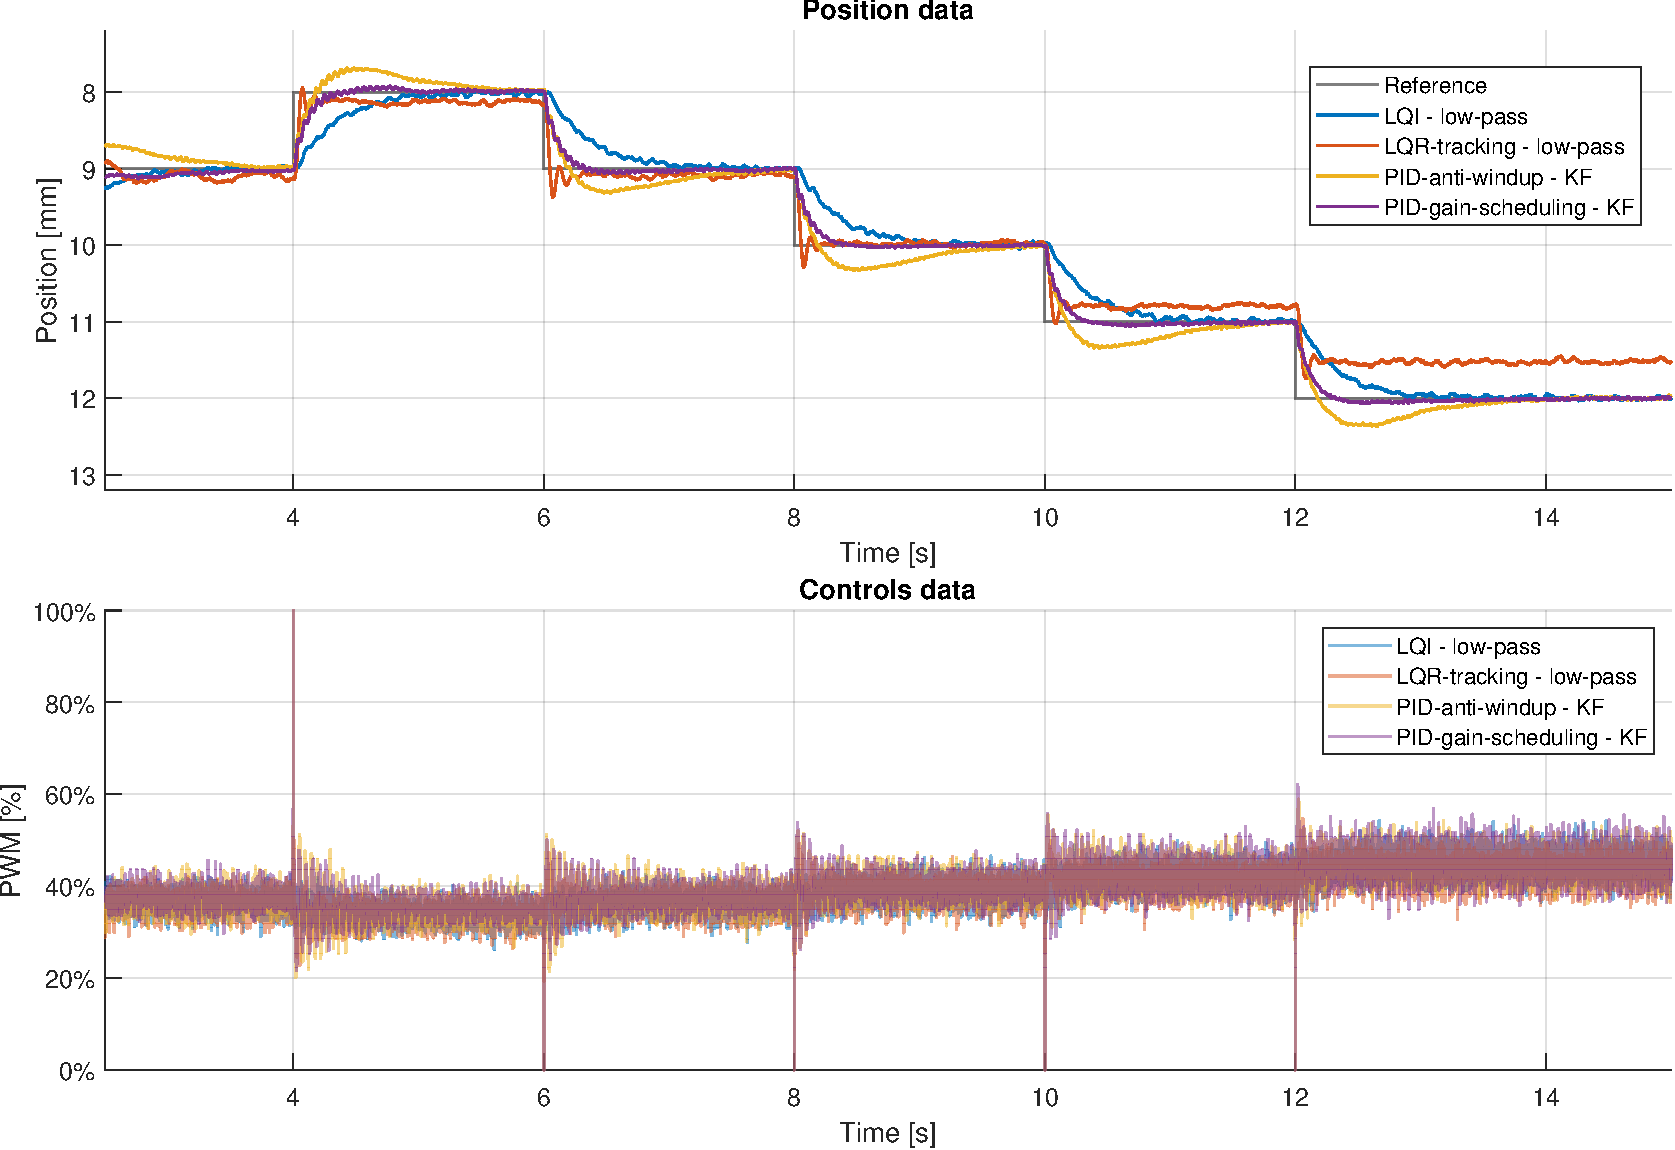
\includegraphics[width=0.8\textwidth]{./img/MATLAB/results/multisteps_stairs_star_star.pdf}
    \caption{Comparison between controllers for multistep reference}
    \label{fig:multistep_1mm}
\end{figure}


\subsection{Response to the sinusoidal reference}
\label{subsec:plot_sinusoidal}

\begin{figure}[H]
    \centering
    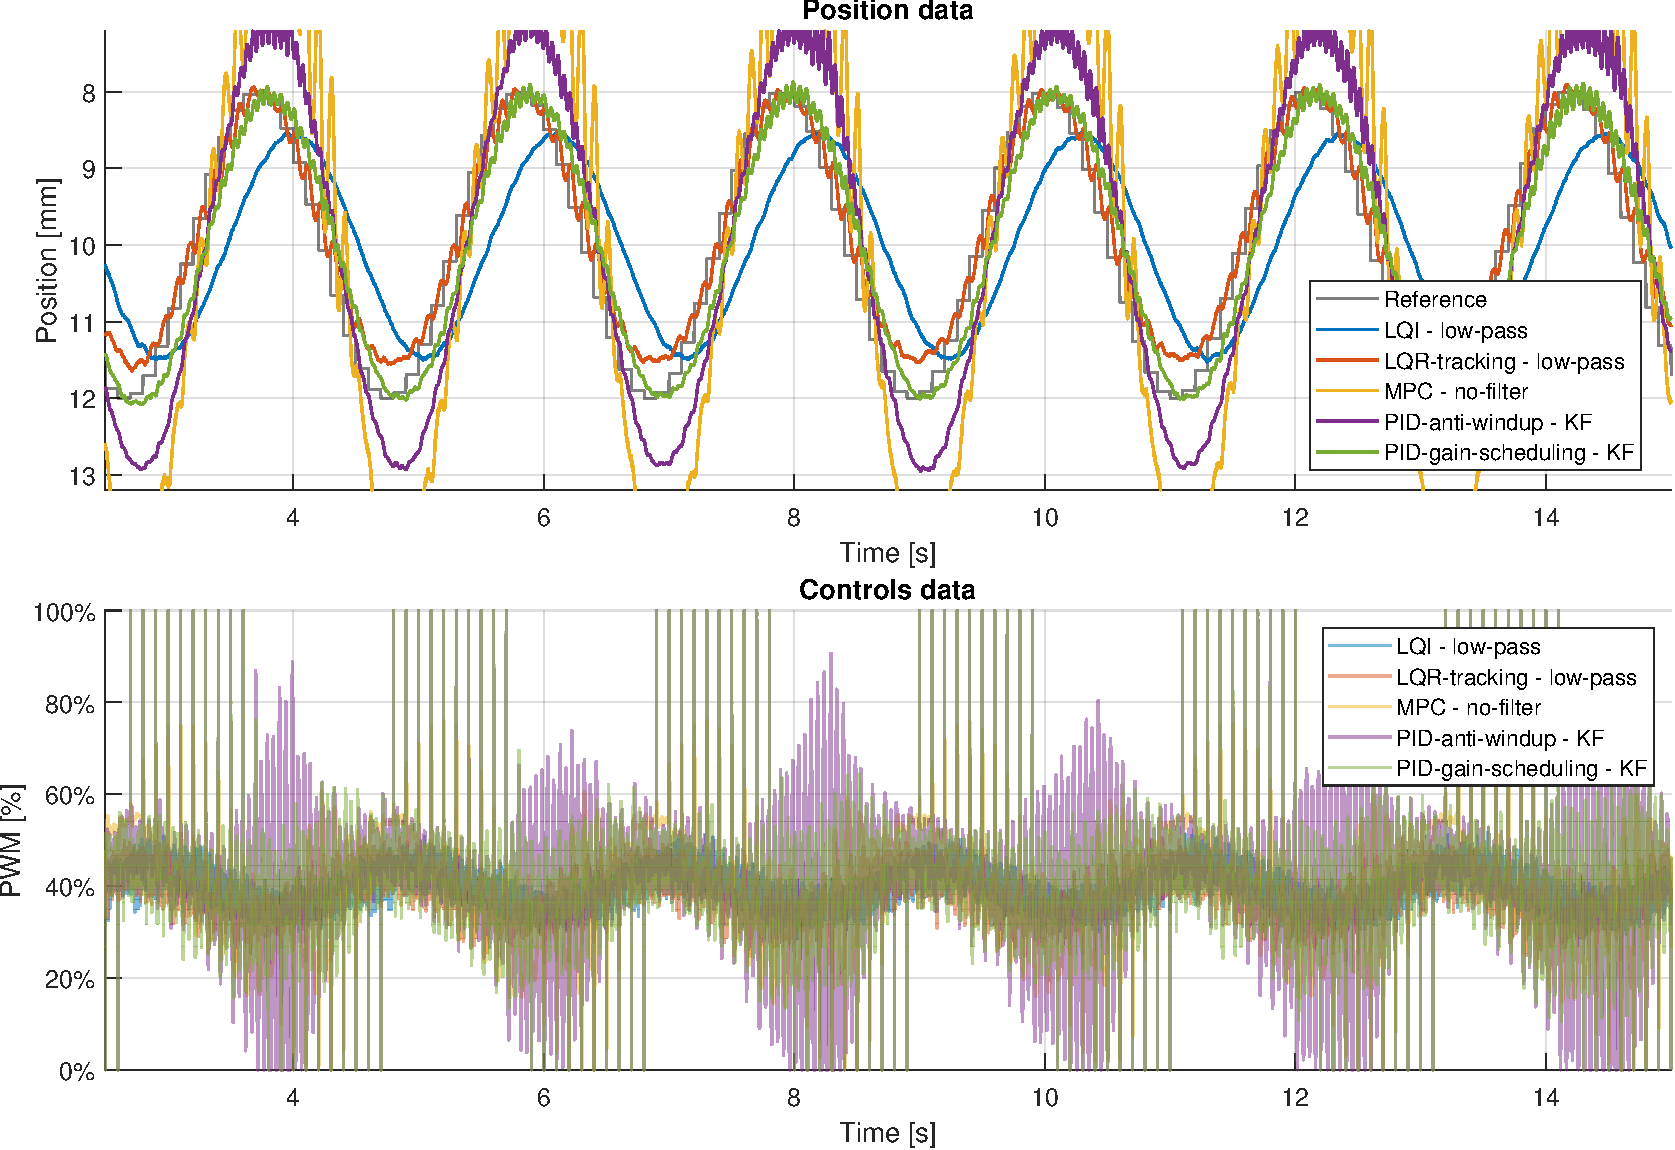
\includegraphics[width=0.8\textwidth]{./img/MATLAB/results/sinusoidal_fast_star_star.pdf}
    \caption{Comparison between controllers for fast sine reference}
    \label{fig:fast_sine}
\end{figure}
\subsection{Comparison of filters}
\label{subsec:plot_filters}

The filters implemented are compared based on the system's response to the fast sinusoidal reference. The controller in the comparison of filters is an LQR tracking controller. The goal is to evaluate the effectiveness and impact of each filtering method on the accuracy of the sphere's trajectory respect to the sinusoidal reference and the quality of the obtained control signal. The compared graphs include the control without filtering, a low-pass filter, a Luenberger observer, a standard Kalman filter, and an extended Kalman filter (EKF).

\textbf{1. Control Without Filters:}
This case represents the least effective way to control the system. Clearly due to the absence of filtering, the system noise is not reduced. Noise filtering, especially for velocity, is critical to achieving accurate response. Using the controller without filters results in imprecise trajectory tracking. The control performance is visibly affected by oscillations and disturbances, making this approach the least suitable for the system under consideration.

\textbf{2. Low Pass Filter:}
Introducing a low pass filter improves the response accuracy compared to the unfiltered case. However, its ability to eliminate noise is limited by the filter's non-adaptive nature, which hinders dynamic performance. The accuracy is higher respect to the case without filters, but lower respect to the other filters, particularly for trajectories requiring rapid variations. To illustrate this behavior, a sinusoidal reference with the minimum period was selected for testing.

\textbf{3. Luenberger Observer:}
The Luenberger observer proves to be more effective than the low pass filter due to its ability to estimate unmeasured system states. However, the control quality remains inferior compared to the Kalman filters. The observer’s performance aligns with expectations, as it does not employ an optimal gain matrix (K) like the Kalman filter.

\textbf{4. Standard Kalman Filter:}
The Kalman filter emerged as the most effective method among those tested. Its ability to optimize state estimation in the presence of measurement and process noise significantly enhances control quality. The trajectory tracking exhibited the highest accuracy with minimal oscillations.

\textbf{5. Extended Kalman Filter:}
Although the EKF is designed to handle system nonlinearities, the results showed inferior performance compared to the standard Kalman filter. Specifically, the EKF failed to adequately follow the reference trajectories. This could be attributed to suboptimal linearizations or poorly tuned covariance matrices. These findings suggest that applying the EKF requires further investigation and optimization to achieve competitive performance.

\textbf{Conclusions:}
The comparative analysis highlighted a clear hierarchy in the performance of the various approaches. The standard Kalman filter stands out as the optimal solution for the analyzed system, ensuring precise and stable control. In contrast, the Luenberger observer and the low-pass filter provide incremental improvements over the unfiltered case but are outperformed by the Kalman filter. Despite its theoretical potential, the EKF delivered unsatisfactory results compared to its simpler counterpart, indicating that it represents a promising area for future research.

These results underscore the importance of selecting appropriate filtering and observation methods in the design of advanced control systems and pave the way for further studies to improve the integration of nonlinear filters in real-world applications.



